\hypertarget{intro}
{\chapter{Introduction}\label{intro}}

This dissertation focuses on how people search for information and how people
rely on this information to inform their health behaviors and develop social
norms. Information permeates every facet of human society, from the hordes of
data gathered through digital-trace data or the passing gossip between friends.
Human communication and human society are based on the circulation of
information and knowledge. Information can be shared and promoted by others
through information campaigns and consumed by an individual, called information
push, or information can be intentionally sought out by individuals, called
information pull \citep{cybenkoFoundationsInformationPush1999}.

We must understand the information individuals receive and seek out to develop a
well-functioning society. The information that one consumes consolidates to
create the entire worldview of every individual, leading to how they understand
the world and behave civilly therein. New and emerging social norms must align
with one's worldview to anticipate any sort of behavioral change, for better or
for worse.

The importance of reputable information and misinformation was clear in the
recent and ongoing COVID-19 pandemic. While the vaccines against the COVID-19
virus are effective in preventing severe illness, hospitalization, and death,
only 60\% of Arizonans over 12 years old \citep{owid} are fully vaccinated
against the virus. We know that people exposed to misinformation are much less
likely to receive vaccinations against the virus
\citep{loombaMeasuringImpactCOVID192021}. It is not an exaggeration to claim
that misinformation has been deadly for Arizona
\citep{pathakInfodemicsCOVID19Role2020, greene_murphy21}.

This dissertation on information search and norm development provides clear and
timely social implications for Arizona and the United States. I uncover how
norms are created during periods of norm uncertainty and builds the foundation
to theorize and test interventions that promote positive norms in times of
disasters and uncertainty. Specifically, I investigate how local diffusion leads
to social norms through information search, which will have strong implications
for the prevention of global polarization and the spread of misinformation, as I
now explain.

In academia and policy, the focus in research on information has always been the
information that is sent to consumers, seeing people as passive receivers of
information. My dissertation instead focuses on individuals as active agents in
their search for information. By looking at how individuals search, I aim to
identify focus areas for future interventions to counter the misinformation
process.

The information that spread to communities in Arizona contributed to the health
behaviors exhibited today by Arizonans. While the information spread in various
ways, including by means of diffusion and polarization, it contributed to our
newly established norms since the Spring of 2020. By uncovering how norms were
created during this time of norm uncertainty, my research will contribute to the
recommended interventions to promote effective health-related behavioral norms
before politicization and misinformation occurs. This will create a healthier,
happier Arizona.

\section{Theoretical Underpinnings}

\subsection{Information Flow}

Humans have long been interested in how to persuade the masses. With the rise of
democracy, the need of the powerful to persuade and appease the masses
dramatically increased. And for a while, behavioral scientists adopted really
simplistic models of persuasion like the assumption that the media influences
behavior in a direct, unmediated, and all-powerful way (termed the hypodermic
needle model in \citet{bineham1988historical}) \citep{lasswellpropaganda}.

A critical turning point in the study of the flow of information was put forth
by renowned sociologist Paul Lazarsfeld and colleagues Verelson and Gaudet
\citeyearpar{lazarsfeldPeopleChoice1944}. They theorized that the media did not
directly influence the masses, but that a ``Two-Step Flow'' was occurring where
``opinion leaders'' interpreted messages from mass media and then, in turn,
promoted their opinions to the masses \citep{katzPersonalInfluencePart1955}. The
opinion leaders interpret, explain, and diffuse contents to ``opinion followers''.
From a networks perspective, ``people rarely act on mass-media information unless
it is also transmitted through personal ties'' \citep[p.
1374]{granovetterStrengthWeakTies1973}. Lazarsfeld et al's
\citeyearpar{lazarsfeldPeopleChoice1944} first study focused on politics, but
follow up studies by \citet{katzPersonalInfluencePart1955} showed that this
model matched information flows beyond the political realm. In contrast to the
one-step flow, where media directly influences the masses, Lazarsfeld's theory
remains in prominence today. While many scholars assumed that modern
micro-targeted marketing strategies would provide evidence for a one-step flow
perspective \citep{bennettOneStepFlowCommunication2006}, many scholars find that
``opinion leaders'' (often influencers and celebrities) still create a two-step
flow of information transmission \citep{choi15, hilbertOneStepTwo2017}.

The spread of information has been thoroughly studied from the perspective of
social networks. Individuals engage with each other and their distributed ties
to create community contexts where norms, beliefs, and values circulate.
Information diffuses through communities and social networks
\citep{fowler2010cooperative, bond_etal12, klarEffectNetworkStructure2017}.
However, ``different things spread in different ways and to different extents''
\citep[p. 563]{christakisSocialContagionTheory2013} and information can spread
differently than a virus or behavior. Important studies in the spread of
information through networks include the study of adoption of innovations by
physicians \citep{colemanDiffusionInnovationPhysicians1957}, how new inventions
are adopted from early adopters to laggards
\citep{rogersDiffusionInnovations1962}, how weak ties help bind networks and
diffuse information \citep{granovetterStrengthWeakTies1973}, how social ties
spread information about job opportunities
\citep{granovetterGettingJobStudy1995, montgomeryJobSearchNetwork1992}, how
information spreads best when weak and strong ties are balanced (embeddedness)
\citep{uzziSocialStructureCompetition1997}, and more recent innovations in the
stickiness of complex contagion \citep{centolaComplexContagionsWeakness2007}.

\subsection{Information Search}
I have only discussed the way that information
is passively consumed through push efforts by opinion leaders and social
networks. However, sociological literature is sparse on the opposite behavior:
active directed searching by individuals to obtain information.
\citet{pejtersenDesignComputeraidedUsersystem1984}, a scholar of library and
information science, theorized that there are 5 strategies for searching for
information. The most common strategy is browsing, where people follow leads
based on associations without planning. Another strategy is analytical, which
includes an explicit consideration of all facets of the question to guide a
search. The empirical method guides the search based on tactics that were
successful in past research. The known site strategy is to go to the direct
source of the information if known. And finally, the similarity method is to
find information based on another similar question that already has an answer.
These 5 strategies vary in their demands for prior knowledge, cognitive
processing, memory, and time spent. While this theory is aimed at finding
information in a library setting, scholars have extended the theory to other
fields and validated the framework \citep{fidelHumanInformationInteraction2012};
the frame is a useful beginning point for the theories of information search
through network activation or through computer-mediated communication.

\subsection{Information Search in The Digital Age}

The introduction of the internet and digital technologies introduced an epochal
disruption in the communication and informational-search mediums that people had
available to them. Computer-mediated communication was the largest communication
revolution in a century, changing the speed and availability of communication
between individuals by electronic mail, instant messaging, two-way interactive
video calls, discussion forums, blogs, and social networking
\citep{rainie2012networked}. Computer-mediated communication encompasses any
sort of communication through computers connected to the internet; the umbrella
term involves both synchronous and asynchronous communication as well as
one-to-one, one-to-many, or many-to-many exchanges. Social media, on the other
hand, are more specific, and are ``Internet-based, disentrained, and persistent
channels of mass personal communication facilitating perceptions of interactions
among users, deriving value primarily from user-generated content'' \citep[][p.
50]{carr2015social}. While an email between colleagues is computer-mediated
communication, it is not social media as there is only one interaction between
users and there is no value derived from the user-generated content outside the
pair \citep{bayer_etal20}. Even more restrictive still is the social networking
site, which consists of a profile, a network, and a stream or a feed
\citep{boyd2007social, ellison2013sociality},  often also involving a messaging
component  \citep{bayer_etal20}. Social networking sites are also interesting
because they often uniquely combine one-to-one communication within the context
of one-to-many communication, like resharing a television news story to your
Facebook feed and chatting with others about the content in the comments
section. But what do these classifications mean for the information-seeking
behaviors of individuals in the 21st century? Not only is it quicker to perform
network activation and seek support, but people are ``permanently online,
permanently connected'' making activation easy \citep{vorderer2017permanently}.
The constant connectedness facilitates communication, but also presents people
with overchoice, or the difficulty in deciding because simply every network
connection you may want to activate is permanently connected and easy to reach.
In other words, constant connection may be debilitating to many who are seeking
information. \citet{smallSomeoneTalk2017} provides many examples of this when he
demonstrates that often, graduate students who needed support simply asked
``miscellaneous classmates encountered down the hall'' (p. 176) rather than their
trusted, long-term confidants. It seems that network activation may rely on more
than just trust; namely: convenience.

The digital age did not only revolutionize communication. It also revolutionized
information search \citep{ramirez2002information}. Just as prior to the digital
age you could open an encyclopedia or peruse the library to find the information
you seek, much of the computer-mediated information search surely occurs outside
of social network activation contexts. While searching in an encyclopedia is far
less common today, internet search engines have revolutionized the speed and
ease at which we can find information. Early web search engines allowed
information seekers to browse web directories, and early engines like Yahoo! and
Altavista found success using keyword-based search, though the early algorithms
were limited in what they could find and relied heavily on the wording of the
queries. Google, the major web search engine used today, introduced the
disruptive PageRank algorithm in the early 2000s, securing its place as the
information hegemon of the 21st century \citep{brin1998anatomy}. Not only has
computer-mediated information search revolutionized the ease of obtaining
information, but it has also changed our brains. \citet{sparrow2011google} show
that the digital age has led to worse memory and higher reliance on technology
to keep track of information for us. These search engines have also shaped our
cultures by controlling, whether through algorithm or intentionally, the
information the engine provides. For example, Google will not show results for
various neo-Nazi websites in countries where holocaust denial is illegal, like
France and Germany. This is illustrative of the control engines have over
information and how this control may introduce various political, economic, and
social biases in the information they provide \citep{segev2010google}. When
99Firms \citeyearpar{99firms22} compiled the data from sources like
NetMarketShare, Statista, DuckDuckGo, Yahoo Finance, Google, and Pew Research
they found that about 93\% of all web traffic is via a search engine and that
78.39\% of all internet searches performed are done using Google. Because
computer-mediated information search is instantaneous and only requires mobile
data or WiFi, there is virtually no cost to seeking information on one of these
mediums.

\subsection{Theory of Uncertainty Management}

Some communication theorists ask why an answer to a question is sought in the
first place. The Theory of Uncertainty Management
\citep{brashersCommunicationUncertaintyManagement2001} professes that people
search for information when their uncertainty around the subject leads to
anxiety or other cognitive harms. The Theory of Motivated Information Management
\citep{afifiSeekingInformationSexual2006, afifiTheoryMotivatedInformation2004}
extends the prior by adding that uncertainty itself is not the catalyst for
information-search; rather, it is driven by a discrepancy between the current
level of uncertainty on a subject and desired level of uncertainty. 
% connect better to social support if possible

\subsection{Social Support}

One way to find information is to activate network ties to find out information
through a form of social support. Social support, while previously used
interchangeably with the term social networks and social integration
\citep{houseStructuresProcessesSocial1988}, consisted of the emotional,
informational, and instrumental assistance functions performed by social ties.
Social support has strong and measurable association with health outcomes
\citep{houseMeasuresConceptsSocial1985, thoitsMechanismsLinkingSocial2011}.
Informational support is the process of seeking ``help in defining,
understanding, and coping with problematic events and include education, advice,
or referral to another source of support'' \citep[p. 640]{winemiller_etal93}.
Brashers, a health communications researcher, defines informational support
slightly differently, focusing on the exchange of information that ``facilitates
coping with life stresses... that may be exchanged among members of a support
network'' \citeyearpar[p. 260]{brashersInformationSeekingAvoiding2002}. Both
definitions provide important lenses for my question of how computer-mediated or
interpersonal information-seeking strategies vary. Some research has revealed
that Facebook users who utilize the platform to find information and to maintain
relationships have high levels of bridging social capital \citep{liu2016meta}.
However, this leaves the question of who activates their social networks for
information using social networking sites like Facebook instead of activating
these networks in face-to-face interactions.


\subsection{Uses and Gratification Theory}

From studies of mass communication, uses and gratifications theory (UGT)
\citep{blumlerUsesMassCommunications1974, tanMassCommunicationTheories1985} may
lend itself to theorizing why information-seeking strategies vary among
different platforms and activation types. UGT posits that users are not passive
consumers of media and that people have an active role in choosing different
sources of media based on their satisfaction of specific needs on an individual
basis. UGT is based on Maslow's \citeyearpar{maslowTheoryHumanMotivation1943}
hierarchy of needs and is compatible with Lazarsfeld and Katz's theory of
two-step flow because people can choose their media and the opinion leaders they
follow. Modern-day theorists have extended UGT theory and classified the uses
and gratifications of the internet and of social media.
\citet{staffordDeterminingUsesGratifications2004} theorize that the internet
provides gratification through useful content that meets expectations,
gratification from purposeful navigating or random browsing as a process, and
social gratification from forming and deepening social ties.
\citet{leungGenerationalDifferencesContent2013} theorizes that social media is
gratifying for users because it allows for venting of negative feelings,
provides recognition, provides entertainment, promotes social affection, and
fulfills cognitive needs.

There has been some research into how different platforms allow for different
user experiences or ``affordances'' \citep{boyd2010social}. For example,
\citet{bossetta18} first show that all social media platforms must provide
``tools that are easy to use and functional to the demands of varying user
demographics'' (p. 473). They also explain how each digital architecture enables,
constrains and shapes how users behave on their platform and in virtual space,
leading to many different experiences along the dimensions of searchability,
connectivity, and privacy.

Adapting UGT to my own purposes, I theorize that informational support will be
activated from network ties when the informational need is accompanied by or
related to a need to form or maintain social ties
\citep{baumeister,grieve2013face}. For instance, Dani, a young college student,
could search on Google to find how to iron their dress shirt properly, but
instead Dani choses to call their parent(s) and ask the best strategy so their
parent(s) feels respected and valued and their relationship is strengthened.
Conversely, I theorize that search will be conducted outside of network
activation when information is needed but an individual does not have an
additional cognitive need to fill through social interaction. For example,
Taylor could ask their neighbor, who is a medical professional about the
newfound headaches they've been experiencing, but every time they talk to their
neighbor they ask for help cleaning their gutters, which is too much work;
Taylor instead may choose to ask the Facebook group they're a part of to gain
information. Alternative goals such as identity management or relational
maintenance \citep{brashersInformationSeekingAvoiding2002} need to be balanced
and may also influence where search is conducted.

\subsection{Social Norms}
I showed that the levels of uncertainty may direct how and when people search
for information. However, in situations of rapidly changing norms, uncertainty
is prevalent. This dissertation also focuses on the development of new social
norms in situations of uncertainty about how to behave. Minimal research exists
in quickly emerging norms in times of emergency but shows that people are likely
to rely on the behavior of others to set their own norms for behavior
\citep{alvarez2018, horneNormsIntegratedFramework2020}. This project
investigates how search contributes to the development of said spontaneous
norms.

Social norms form the building blocks of social organization and have been a
focus of sociology since the beginning. In a 2020 Annual Review of Sociology
piece focused on social norms, Horne and Mollborn define norms as ``group-level
evaluations of behavior ... [or] when people have expectations about how others
evaluate behaviors'' \citeyearpar[p. 468-69]{horneNormsIntegratedFramework2020}.
One of the principal architects of sociology, \'{E}mile Durkheim, saw that
society exerted powerful forces on individuals and classified people's norms,
beliefs, and values as parts of collective consciousness that provide for
societal integration \citeyearpar{durkheimSuicide1897,
durkheimDivisionLaborSociety1933}. For Durkheim, norms were therefore the glue
that held society together in cohesion.

Max Weber, another founding architect of sociology saw social norms differently.
Weber distinguished social behavior from social action, which was an action a
person takes through subjective understanding and interpretation of actions of
others \citeyearpar{weber1978economy}. Weber therefore saw social norms through
the lens of the subjective meanings behind every action. Actions that were not
considered by an individual were not the focus of Weber. New spontaneous norms
that are emerging in a society under upheaval, like the health behaviors that
emerged during the COVID-19 pandemic, emerged with new subjective meanings and
cognitive associations that held consequences for the individuals who adopted
the social actions.

The causes and logics of social norms are debated. The consequentialist argument
for norms focuses merely on the consequence a behavior has on group members and
that norms will be promoted if the behavior benefits others and denounced if it
negatively affects others \citep{ullmannmargalitEmergenceNorms1977}. While this
theory has been tested and performs well in the lab, researchers have raised
questions regarding its ecological validity
\citep{horneNormsIntegratedFramework2020}. One of the main critiques of the
consequentialist argument is that it relies on the same interpretation of the
perceived action by all parties of what is harmful and beneficial. The
Relational argument for norms is based on the value people place on their
relationships and the assumption that people will behave in ways that will
garner them positive social reactions. This argument relies on individuals
assuming what their peers will approve and disapprove of. In turn, norms are
developed when individuals make inferences from their social worlds
\citep{fryeCulturalMeaningsAggregation2017}. Importantly, people look to others
performing an action and often interpret that performance as an indication that
an action is approved, paying particular attention to high-status individuals
and institutions \citep{robalinoPeerEffectsAdolescent2018,
tankardEffectSupremeCourt2017}.

\subsection{Social Networks}

Norms are formed inside of social networks; ``Networks operate in a larger
cultural context that can facilitate or inhibit acceptance of general cultural
norms and beliefs'' \citep[][p. 44]{pescosolidoDurkheimSuicideReligion1989}.
Because of this, people tend to resemble their network as a form of network
autocorrelation and homophily \citep{dellapostaWhyLiberalsDrink2015}. While
``birds of a feather flock together'' in homophily
\citep{mcphersonBirdsFeatherHomophily2001}, attitudes and behaviors are shaped
by peers, creating filter bubbles of social influence
\citep{dellapostaWhyLiberalsDrink2015}.

\citet{goldbergSocialContagionAssociative2018} argue that the state of the
literature on diffusion and social contagion, discussed above, is erroneous.
They propose an important linkage that had been missed in previous research of
the diffusion of behavior (or, as I interpret it, the creation of new norms).
They argue that what actually diffuses during social contagion are the
perceptions about which beliefs or behaviors are compatible with one another,
what they call ``associative diffusion''. This relates back to the theory of
relational norms, where individuals assume what their peers will approve and
disapprove of. For these assumptions to take place, they must understand which
behaviors and beliefs are possessed by whom in their network and how new
associations may influence or disrupt the expected actions. In times of
behavioral uncertainty, I theorize that individuals strategically look towards
other high-status individuals and institutions, and perform regimented searches
to establish for themselves the behavior that is compatible with other cognitive
associations and biases they hold.

\section{Three Empirical Articles}

To investigate information-seeking behaviors, online search tools, and how new
norms in health behaviors form, I first provide an outline of the information
push and pull process in Figure \ref{fig:concept-map}. After being exposed to
new information, an actor can choose to further investigate the information if
their level of uncertainty on the subject surpasses the desired level of
uncertainty \citep{brashersCommunicationUncertaintyManagement2001}. Search can
then be performed online or offline and be pushed further to the actor's
networks.


\begin{figure}
{\centering 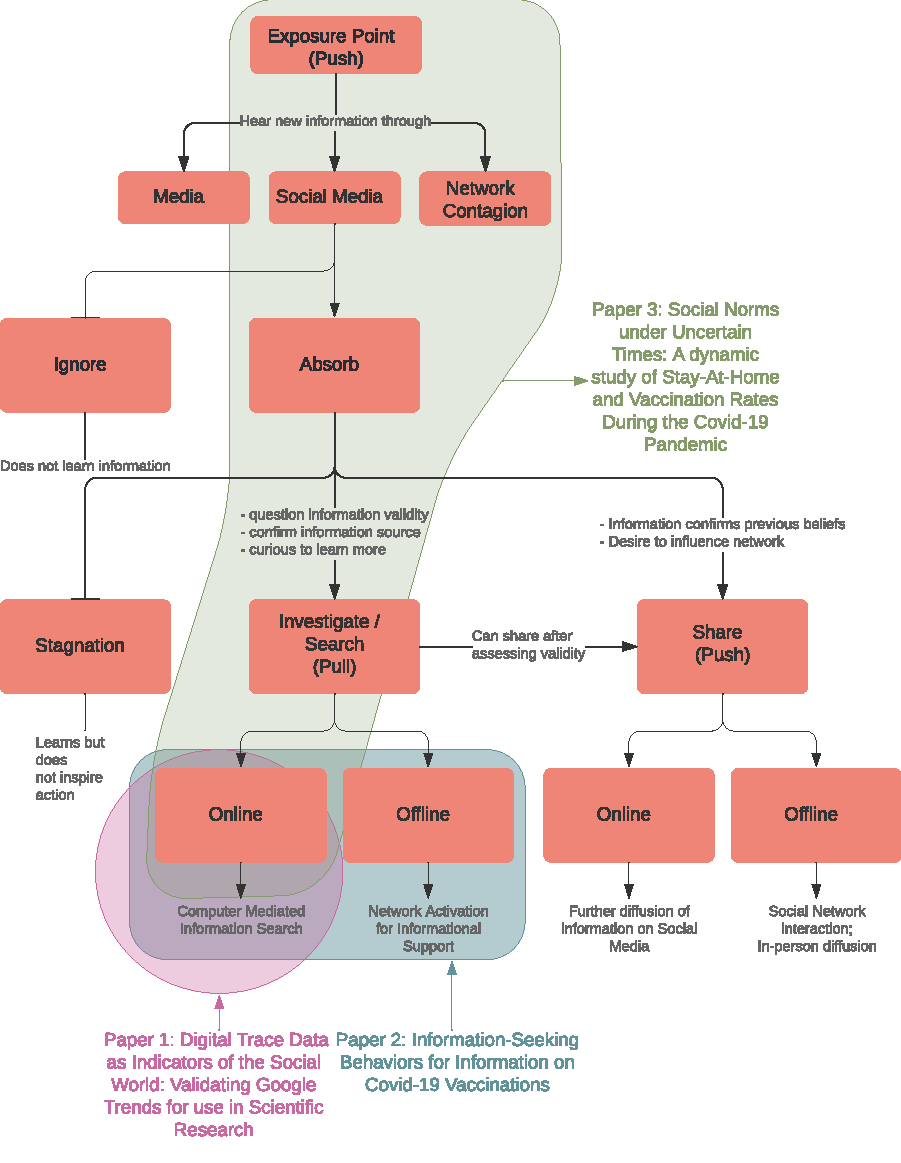
\includegraphics[width=\linewidth]{figs/ch1/Dissertation Concept Map - Color.pdf}}
\caption{Theoretical Framework for the Dissertation}\label{fig:concept-map}
\end{figure}

This dissertation uses three articles to investigate different parts of the
theoretical framework (Figure \ref{fig:concept-map}). The dissertation is
divided into three parts, with Article 1 focusing on online information search,
Article 2 focusing on online and offline information search, and Article 3
investigating the entire information push and pull process in the context of
establishing new norms.

\hyperlink{paper-1}{\subsection{Article 1: Digital Trace Data as Indicators of the Social World: Validating Google Trends for use in Scientific Research}}

Computational social science and social science disciplines are quick to adopt
new sources of digital trace data for use in academic research. In this article,
I examine the criterion validity of one of these new sources, Google Search
Trends. Criterion validity looks at how well an operationalization of a specific
construct is able to predict a theoretical representation of the construct — the criterion.
I validate how Google Trends can be used as an operationalization of three different
cases, namely attitudes, disease prevalence and political preferences using five
different validated data sources. This paper asks, ``How can we operationalize
Google Search Trends as a valid indicator for uses in social science research?''
I use Pearson and Repeated Measures Correlations between the Google Trends and
the validated indicators as well as multiple linear regression (for
cross-sectional datasets) and fixed effect hierarchical linear models (for
longitudinal datasets) as additional tests of the data.

I find no correlation among any of the Google Trends tested and their validated
indicators. While some Google Trends tested were significantly associated with
the outcome in the regression models, effects tended to be small and the total
model interpretability remained low, even when controlling for demographic
variables. This article shows that there is no criterion validity of
Google Trends for these uses and social scientists will find no replacement for
high quality survey data with Google Trends. Instead, we must only use Google
Trends to demonstrate interest or attention.

\hyperlink{paper-2}{\subsection{Article 2: Information-Seeking Behaviors for Information on COVID-19 Vaccinations}}

Knowing that Google trends data only encompasses a small portion of the
information-seeking done by modern humans, it is important to investigate what
leads individuals to search for a question online using a search engine versus
more traditional means of information gathering, such as network activation
(asking someone in their social network for informational support). Previous
research has greatly failed to distinguish between the activation of information
seeking behaviors online and offline. Using theories of social support and uses
and gratifications theory, I investigate the factors associated with each
information seeking modality: personal connection, doctor, social networking
site, online forum, and online search engine. I use original survey data of 948
Americans to investigate their experiences seeking out information about the
COVID-19 vaccines.

This paper aims to address two main questions:
\begin{itemize}
  \item How do computer-mediated or interpersonal information-seeking strategies vary
across populations?
  \item How does the information search modality utilized affect COVID-19 Vaccination uptake? 
\end{itemize}

In this article, I find little evidence that online search is more utilized than
seeking social support from personal network connections or health professionals
as I hypothesize based on uses and gratifications theory. I find evidence that
the categorizations of modalities queried in this survey are indeed conceptually
different from each other and that the utilization of different modalities
varies by demography and information exposure points. Finally, I find that
different exposure points and information search modalities hold real world
consequences through their associations with COVID-19 vaccination rates and
intentions, as information from a doctor increases the COVID-19 vaccination
uptake while receiving information from a social networking site like Facebook
or Twitter was associated with lower odds of vaccination.

\hyperlink{paper-3}{\subsection{Article 3: Social Norms under Uncertain Times: A dynamic study of Stay-At-Home and Vaccination Rates During the COVID-19 Pandemic}}

My final article takes a deeper dive into the formation of social norms
governing health behaviors in cases of extreme uncertainty using the cases of
both stay-at-home rates and vaccination rates as responses to public health
recommendations to mitigate the COVID-19 pandemic. Using theories like
associative diffusion and the integrated theoretical framework of norms, I test
models of behavioral adaption to public health recommendations and patterns of
complex contagion (the need for repeated exposures to something novel for it
to diffuse) using linear mixed effects models.

These models show that complex contagion is a valid framework for the social
contagion of new norms during COVID-19. Importantly, I find a novel moderating
effect of signal discordance, the contextual diversity of signals received by an
ego. If there is diversity in the information received by an ego, contagion is
less likely to occur. This paper shows that the contagion process cannot be
fully understood without looking at the context of each exposure to a contagion
within the range of contagions one experiences.


\section{Contributions and Future Directions}

% search as an agentic process
This research makes contributions to multiple subfields and literatures. First
and foremost, these articles contribute to the sociological literature. The
spread of information has long been investigated in the discipline (diffusion,
mass communication, social influence). However, it is almost always researched
from a structural perspective which disregards individual agency and choice in
the acquisition of new information. This dissertation adopts the second
perspective, centering people as active agents in their search for information
aligned with their own preferences and gratifications instead of just passive
receivers of information signals. Taking this agentic perspective is critical in
the study of information diffusion when combined with cognitive perspectives
like that of \citet{goldbergSocialContagionAssociative2018}. How people search
for information is a strong determinant of the information that they find. The
information they uncover is filtered through cognitive biases and
predispositions to how they interpret and act upon the newfound information.
Searching for informational support through social network ties theoretically
will uncover potentially different information than would be found through
online web search and will change how people are organized and how people
behave. \hyperlink{paper-2}{Article 2}, for instance, demonstrates that the
choice to receive a COVID-19 vaccine is impacted by how individuals search for
information on the vaccine. This is a real-world consequence to the variation in
the individual information search process.

% CSS & big data
This dissertation also contributes to computational social science \& critical
big data studies. In two articles, I employ Google Search Trends which are
relatively underutilized in the social sciences compared to health sciences and
business. Because \hyperlink{paper-1}{Article 1} takes a critical big data
studies approach, I consider the potential pitfalls that any source of big data
face \citep{mcfarlandBigDataDanger2015} and explicitly test just how well Google
Trends can be used as an indicator for different concepts through criterion
validity. Importantly, I find that Google Trends cannot replace high quality
survey data. This is a large contribution to the field of critical big data
studies but also provides the groundwork for future tests of external validity
for big data for future computational social scientists.

% micro behaviors to macro processes
Bridging the contribution of search as an agentic process and critical big data
studies, this dissertation contributes to the question posed by
\citet{breigerScaling2015}, ``what are the behavioral processes that lead to
macro-level outcomes?'' With the exponentially growing size of digital-trace data
that is available, it is important to not only uncover the external and
criterion validity of the data and correspondence to real world behaviors (see
\hyperlink{paper-1}{Article 1}) but also important to understand the social
forces that lead to the big data. One of the contributions of
\hyperlink{paper-2}{Article 2} is to dive deep into this question, uncovering
why some people choose to use web search engines over other information search
modalities. These papers are a first step in validating and establishing a
deeper understanding of who the users are that contribute to macro-level
aggregate trends.

% social norms
Additionally, this dissertation investigates how social norms are formed in
situations of uncertainty, an area that is far less developed in sociology.
While sociologists have studied social norms since the formation of the
discipline, norms are most often studied under the lens of the emergence of
norms and transmission of norms between groups, deviance and social control, the
interaction of norms as ``mental representations of appropriate behavior''
\citep{aarts2003silence}, and research categorizing different types of norms
(e.g.\, descriptive versus injunctive, prescriptive versus proscriptive). The
focus on the formation of new social norms during times of uncertainty has
implications for interventions in social behavioral outcomes, research on
cultural change, and the spread of cognitive associations. Moreover,
\hyperlink{paper-3}{Article 3} focuses on how conflicting behaviors become
settled into cognitive associations, providing a relevant framework for research
on unrest and disasters.

% social networks / diffusion
This dissertation also has implications for the study of social networks and
diffusion. \citet{centolaComplexContagionsWeakness2007} introduced a pivotal
disruption to the diffusion literature when they developed complex contagion,
the need for reinforcement through multiple exposures.
\hyperlink{paper-3}{Article 3} in this dissertation takes this disruption one
step further to demonstrate that the concordance of the exposure affects the
contagion process; in other words, being exposed to a diversity of diffusants
(discordance) can prevent the diffusant from spreading. This critical finding
provides many new areas of exploration for scholars to further investigate the
interdependence between different beliefs that are diffusing and under what
contexts the discordance matters.

% social epidemiology
I also make important contributions to social epidemiology through this research
with the use of health case studies for questions of sociological interest
across my three articles. Because of this, I contribute to the social
epidemiological conversation on vaccine hesitancy, health communication, and
diffusion of high-risk health behaviors. While all these areas are important to
social epidemiology, they hold potential important health implications for these
contributions on outside of the academy, covered in the first paragraphs of this
chapter.

%  polarization misinformation
% This work also relates to polarization and misinformation, two major
% social issues of our time. \citet{axelrodDisseminationCultureModel1997} shows that network structure,
% autocorrelation, and diffusion create local convergence of attitudes and
% culture which then leads to global polarization \citep{dellapostaWhyLiberalsDrink2015}. In investigating how local diffusion leads to social norms
% through information search, some of my findings may have strong
% implications and interventions for the prevention of global
% polarization. Relatedly, understanding where and how people search for
% information has implications for the information they are exposed to and
% the norms they develop. This project will attempt to relate to where
% misinformation is uncovered and how to intervene in its absorption.